% Conversion of EPS graphics with psfrag annotations into PDF
% run with
% latex <filename>.tex && dvipdf <filename>.dvi => filename.pdf
\documentclass[12pt,a4paper]{article}
\usepackage[english]{babel} 
\usepackage[latin1]{inputenc}   
\usepackage[T1]{fontenc} 		
\usepackage{amsmath}
\usepackage{amssymb}
\usepackage{latexsym}

\usepackage[active,tightpage]{preview}
\setlength\PreviewBorder{5pt}

\usepackage[dvips]{graphicx}
\usepackage{xcolor}
\usepackage{psfrag}
\usepackage{pstricks,pst-node}

\begin{document}
\begin{preview}
  \begin{minipage}[c]{\textwidth}
    \centering
    \psfrag{L1}[l][l]{\small {$L$}}
    \psfrag{R1}{\small {$R$}}
    \psfrag{R2}[c][c]{\small {$R$}}
    \psfrag{C1}{\small {$C_{1}$}}
    \psfrag{C2}{\small {$C_{2}$}}
    \psfrag{R3}{\small {$R$}}
    \psfrag{R4}{\small {$R$}}
    \psfrag{R5}[c][c]{\small {$R$}}
    \psfrag{Rx}{{$R_{x}$}}
   %  \psfrag{1}{}
   %  \psfrag{2}{}
   %  \psfrag{3}{}
   %  \psfrag{4}{}
   %  \psfrag{5}{}
   %  \psfrag{6}{}
   % \psfrag{7}{}
   %  \psfrag{8}{}
   %  \psfrag{9}{}
   %  \psfrag{10}{}
   %  \psfrag{11}{}
   %  \psfrag{13}{}
   %  \psfrag{14}{}
   %  \psfrag{15}{}
   %  \psfrag{16}{}
   %  \psfrag{17}{}
   %  \psfrag{18}{}
    \psfrag{U}{{$U$}}
    \psfrag{Rx}{{\color{magenta}$R_{x}$}}
    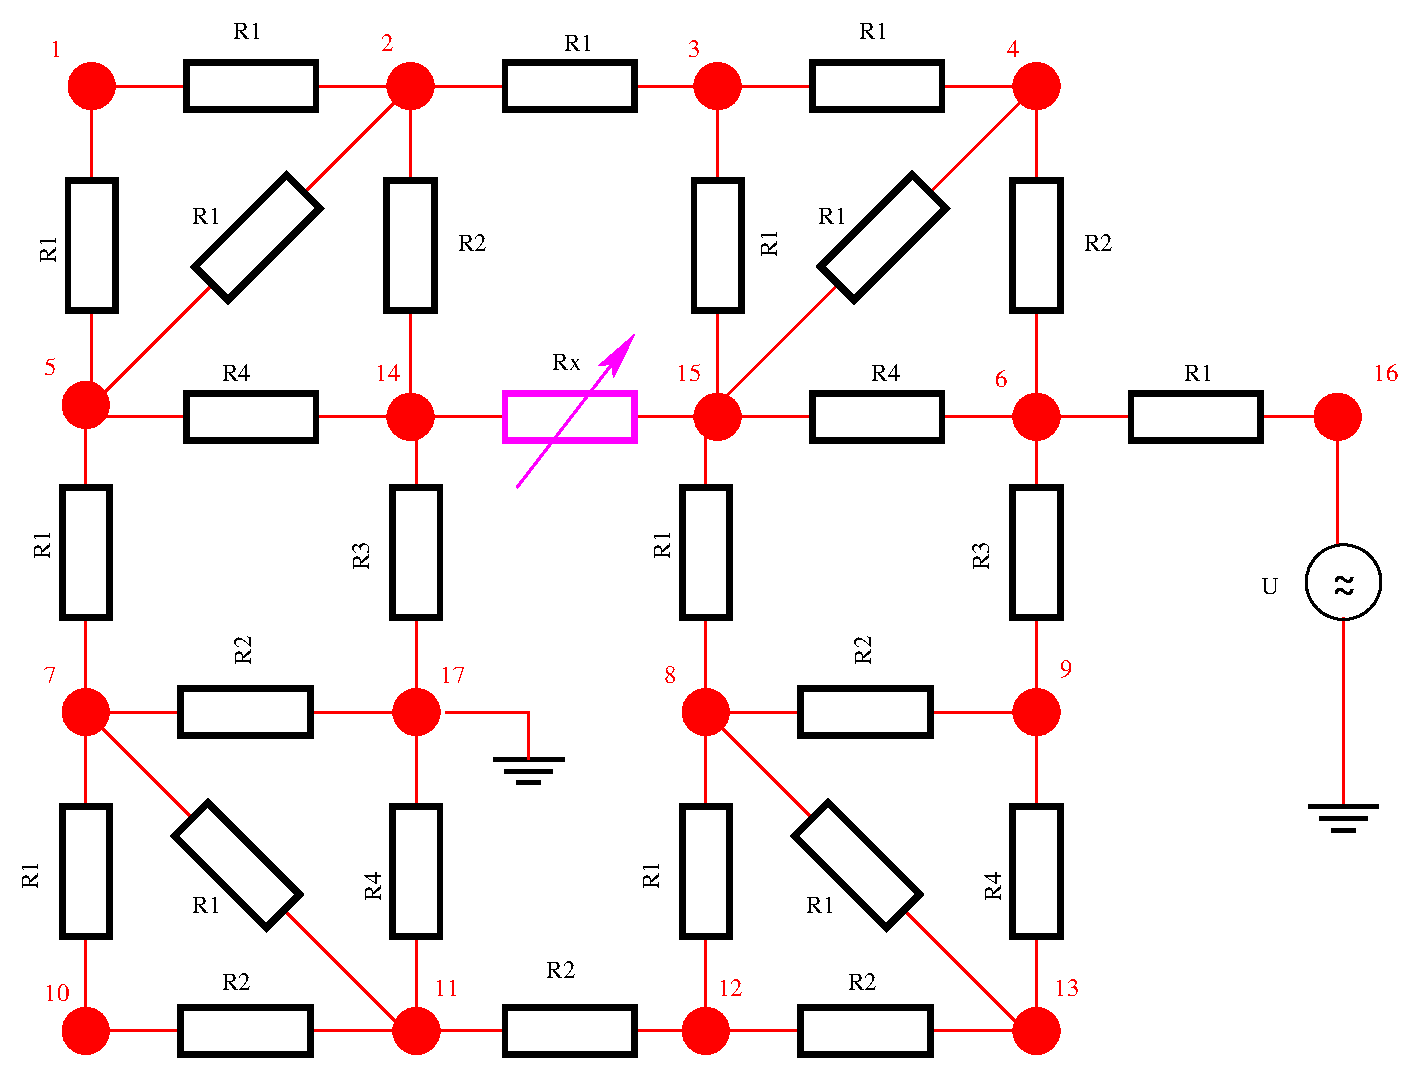
\includegraphics[width=0.75\textwidth]{./PICTURES/rcircuit.eps}
  \end{minipage}
\end{preview}
\end{document}
